%%% License: Creative Commons Attribution Share Alike 4.0 (see https://creativecommons.org/licenses/by-sa/4.0/)

\documentclass[english,10pt
,aspectratio=169
%,handout
%%%%%%,notes
]{beamer}
%%% License: Creative Commons Attribution Share Alike 4.0 (see https://creativecommons.org/licenses/by-sa/4.0/)

\DeclareGraphicsExtensions{.eps, .pdf,.png,.jpg,.mps,}
\usetheme{reMedian}
\usepackage{parskip}
\makeatother

\renewcommand{\baselinestretch}{1.1} 

\usepackage{amsmath, amssymb, amsfonts, amsthm}
\usepackage{enumerate}
%\usepackage{enumitem}
\usepackage{hyperref}
\usepackage{url}
\usepackage{bbm}
\usepackage{color}

\usepackage{tikz}
\usepackage{tikzscale}
\newcommand*\circled[1]{\tikz[baseline=(char.base)]{
		\node[shape=circle,draw, inner sep=-20pt] (char) {#1};}}
\usetikzlibrary{automata,positioning}
\usetikzlibrary{decorations.pathreplacing}
\usepackage{pgfplots}
\usepgfplotslibrary{fillbetween}
\usepackage{graphicx}

\usepackage{setspace}
\thinmuskip=1mu
\medmuskip=1mu 
\thickmuskip=1mu 


\usecolortheme{default}
\usepackage{verbatim}
\usepackage[normalem]{ulem}

\usepackage{apptools}
\AtAppendix{
	\setbeamertemplate{frame numbering}[none]
}
\usepackage{natbib}


% red strikeout
\newcommand\soutred{\bgroup\markoverwith
	{\textcolor{red}{\rule[0.55ex]{2pt}{0.8pt}}}\ULon}



% To use LyX frames from old version:
\def\lyxframeend{} % In case there is a superfluous frame end
\long\def\lyxframe#1{\@lyxframe#1\@lyxframestop}%
\def\@lyxframe{\@ifnextchar<{\@@lyxframe}{\@@lyxframe<*>}}%
\def\@@lyxframe<#1>{\@ifnextchar[{\@@@lyxframe<#1>}{\@@@lyxframe<#1>[]}}
\def\@@@lyxframe<#1>[{\@ifnextchar<{\@@@@@lyxframe<#1>[}{\@@@@lyxframe<#1>[<*>][}}
\def\@@@@@lyxframe<#1>[#2]{\@ifnextchar[{\@@@@lyxframe<#1>[#2]}{\@@@@lyxframe<#1>[#2][]}}
\long\def\@@@@lyxframe<#1>[#2][#3]#4\@lyxframestop#5\lyxframeend{%
	\frame<#1>[#2][#3]{\frametitle{#4}#5}}


\title{Mechanism Design}

\subtitle{5: Beyond the Euclidean setting}

\author{Egor Starkov}

\date{K{\o}benhavns Unversitet \\
	Fall 2022}


\begin{document}
	\AtBeginSection[]{
		\frame{
			\frametitle{This slide deck:}
			\tableofcontents[currentsection,currentsubsection]
	}}
	\frame[plain]{\titlepage}



\section{Testing Implementability}

\begin{frame}{Testing Implementability}
	\begin{exampleblock}{}
		How can we check whether a given $f(\theta)$ is implementable?
	\end{exampleblock} 
	\begin{itemize}
		\item We have seen an answer for the Euclidean setting (monotonicity). What about more general settings?
	\end{itemize}
\end{frame}


%\begin{frame}{DSIC: Weak Preference Reversal Property}
%	\begin{itemize}
%		\item \textbf{Answer 1}: \structure{revelation principle}. (Applies to any \alert{general} setting.)
%		Construct a DRM and check all players' \alert{IC conditions}; s.c.f. is implementable iff it satisfies them:
%		$$ u_{i}(f(\theta_{i}', \theta_{-i}), \theta_{i}') \geq u_{i}(f(\theta_{i}'', \theta_{-i}), \theta_{i}') \text{ for all } i,\theta_i',\theta_i'',\theta_{-i}.$$
%		
%		\item Note that they imply the following \structure{preference reversal} condition: for all $i,\theta_i',\theta_i'',\theta_{-i}$,
%		\begin{align*}
%			u_{i}(f(\theta_{i}', \theta_{-i}), \theta_{i}') &\geq u_{i}(f(\theta_{i}'', \theta_{-i}), \theta_{i}'),
%			\\
%			u_{i}(f(\theta_{i}', \theta_{-i}), \theta_{i}'') &\leq u_{i}(f(\theta_{i}'', \theta_{-i}), \theta_{i}'').
%		\end{align*}
%		\item $i$'s preference between $f(\theta_{i}', \theta_{-i})$ and $f(\theta_{i}'', \theta_{-i})$ should flip when his type changes from $\theta_i'$ to $\theta_i''$ for $f$ to be DSIC. In other words:
%		\item ``To each their own'': different types should get their most preferred option among the available ones.
%	\end{itemize}
%\end{frame}


\begin{frame}{Monotonicity: Euclidean setting}
	\begin{itemize}
		\item \textbf{Reminder}: \structure{monotonicity} for Euclidean problems.
		\begin{itemize}
			\item Note: only the players' preferences are required to be linear for this to hold; the principal can have non-linear prefs. 
		\end{itemize}
		\item In a \alert{Euclidean} setting, $k(\theta)$ is implementable only if it is monotone.
		\item Turns out, this is a sharp characterization: \\
		if $k(\theta)$ is monotone, there exist transfers $t$ such that $\Gamma = (\Theta, (k,t))$ is DSIC.
		\begin{itemize}
			\item Monotonicity may require $k(\theta)$ to be either weakly increasing, or weakly decreasing, depending on the problem.
			\item To prove: use the relevant ERP to construct all transfers; can then show that the resulting mechanism is DSIC/BIC as needed.
		\end{itemize}
	\end{itemize}
\end{frame}


%TODO: add also a convex v result


\begin{frame}{Monotonicity: quasilinear setting}
	Extension to \alert{quasilinear} setting:
	\begin{exampleblock}{Definition (\textbf{weak q-monotonicity})}
		Allocation $k$ is \alert{weakly q-monotone} if for all $i,\theta_i',\theta_i'',\theta_{-i}$:
		\begin{equation*}
			v_{i}(k(\structure{\theta_{i}'}, \theta_{-i}), \structure{\theta_{i}'}) - 
			v_{i}(k(\alert{\theta_{i}''}, \theta_{-i}), \structure{\theta_{i}'}) 
			\geq 
			v_{i}(k(\structure{\theta_{i}'}, \theta_{-i}), \alert{\theta_{i}''}) - 
			v_{i}(k(\alert{\theta_{i}''}, \theta_{-i}), \alert{\theta_{i}''}) 
		\end{equation*}
	\end{exampleblock}
	\begin{theorem}[Necessity of weak monotonicity in qlin setting]
		In the quasilinear setting: if $k$ is DSIC then $k$ is weakly q-monotone.
	\end{theorem}
	So $k$ must be weakly q-monotone to be implementable.\\ 
	But weak q-monotonicity does not guarantee implementability. \\
	But we can strengthen this...
\end{frame}


\begin{frame}{Monotonicity: quasilinear setting}
	\begin{exampleblock}{Definition (\textbf{cyclical q-monotonicity})}
		Allocation $k$ is \alert{cyclically q-monotone} if for all $i,\theta_{-i}$, and all sequences $(\theta_i^1,\theta_i^2,...,\theta_i^M)\in \Theta_i^M$ of arbitrary length $M$ s.t. $\theta_i^M=\theta_i^1$, the following holds:
		\begin{equation*}
			\sum_{m=1}^{M-1}
			\left[
			v_{i}(k(\alert{\theta_{i}^m}, \theta_{-i}), \alert{\theta_{i}^{m+1}}) - 
			v_{i}(k(\alert{\theta_{i}^{m}}, \theta_{-i}), \alert{\theta_{i}^m}) 
			\right] 
			\leq 0
		\end{equation*}
	\end{exampleblock}
	\begin{theorem}[\textbf{\citet{rochet_necessary_1987}}]
		In a quasilinear setting: $k$ is DSIC if and only if $k$ is cyclically q-monotone.
	\end{theorem}
	\textbf{Note}: ``Weak q-monotonicity'' = ``cyclical q-monotonicity for $M=3$''.
	See B{\"o}rgers, ch.5.3-5.4 for proofs or references to proofs (for $N=1$). See rest of ch.5 for other kinds of monotonicity for quasilinear setting.
\end{frame}


\begin{frame}{Monotonicity: general setting (1)}
	\textbf{Without transfers}, interesting results come up... 
	\begin{exampleblock}{Definition (\textbf{outcome g-monotonicity})}
		In a general setting, outcome $x$ is \alert{g-monotone} if for all $\theta',\theta'' \in \Theta$ the following holds:
		\begin{itemize}
			\item if for all $i$ and all $x' \in X$ s.t. $u_i(x(\theta'),\theta') \geq u_i(x',\theta')$ it holds that $u_i(x(\theta'),\theta'') \geq u_i(x',\theta'')$,
			\item then $x(\theta'')=x(\theta')$.
		\end{itemize}
	\end{exampleblock}
	In words, if under $\theta''$ everyone likes $x(\theta')$ more than under $\theta'$, then we give $x(\theta')$ under $\theta''$.
	\begin{theorem}[Necessity of monotonicity in general setting]
		In the general setting: if $x$ is DSIC and $x(\Theta)=X$ then $x$ is g-monotone.
	\end{theorem}
	(This is not THE interesting part yet. The next result is.)
\end{frame}


\begin{frame}{Monotonicity: general setting (2)}
	%\textbf{Assume} $X$ is finite and 
	\begin{exampleblock}{Assumption (\textbf{Domain})}
		Assume type sets $\Theta_i$ are rich enough to contain all possible (ordinal) preferences over $X$ for all $i$.
	\end{exampleblock}
	\begin{exampleblock}{Definition (dictatorial s.c.f.)}
		S.c.f. $f$ is called \alert{dictatorial} if there exists $i \in N$ s.t. for all type profiles $\theta$:
	$ f(\theta) \in \arg \max_x u_i(x,\theta_i).$
	\end{exampleblock}
\end{frame}


\begin{frame}{Monotonicity: general setting (3)}
	\begin{theorem}[\textbf{\cite{gibbard_manipulation_1973,satterthwaite_strategy-proofness_1975}}]
		In a general setting with $|X|\geq 3$: if $x(\Theta)=X$, then\\
		\centering
		$x$ is \alert{DSIC} if and only if $x$ is \alert{dictatorial}.
	\end{theorem}
	\begin{itemize}
		\item To clarify, $x(\Theta) \equiv \left\{ x \in X \mid \exists \theta: x(\theta) = x \right\}$ is the set of ``outcomes that could be prescribed for some $\theta \in \Theta$''.
		\item Note: restriction $x(\Theta) = X$ is irrelevant.\\
		If $x(\Theta) \subset X$, then only preferences over alternatives in $x(\Theta)$ are relevant, and we will still have a dictatorship on $x(\Theta)$. This is something we'll come back to later.
		\item GS theorem is the mechanism design version of Arrow's theorem from social choice.
	\end{itemize}
\end{frame}


\begin{frame}{Monotonicity: general setting (4)}
	\begin{itemize}
		\item The missing link between the two results above is this:
		\begin{theorem}[Monotonicity implies dictatorship]
			In a general setting with $|X|\geq 3$: if $x(\Theta)=X$ and the domain assumption hold, then\\
			\centering
			if $x$ is g-monotone then $x$ is dictatorial.
		\end{theorem}
		\item For a full proof of GS thm, see B{\"o}rgers, ch.8.2, or \cite{svensson_proof_2014}
		\item All three results for the general setting hold with ordinal preferences ($\succsim_i$) too, they do not rely on cardinal utilities $u_i$.
		%\begin{itemize}
		%	\item If anything, the domain assumption ($x(\Theta)=X$) is easier to state with ordinal preferences.
		%\end{itemize}
		\item The GS thm is also extendable to infinite $X$.
	\end{itemize}
\end{frame}


\begin{frame}{Monotonicity: general setting (5)}
	\begin{itemize}
		\item It \emph{seems} like GS thm is a strong negative result saying ``we can't implement anything unless it's dictatorial!''. But we obviously can: we've seen examples (like VCG). Where is the contradiction?
		\item The source of evil in GS thm is the \alert{domain} assumption (``any preference is possible''). \\
		We often know \structure{something} about some players' preferences, so can restrict the set of possible preferences.
		\begin{itemize}
			\item E.g., quasilinear prefs: ``everyone always likes money''. Then at least the efficient allocation rule $k^*(\theta)$ is implementable (and typically not dictatorial!)
			\item Another common example is the single-peaked preferences. They also allow for non-dictatorial DSIC mechanisms. (B{\"o}rgers, Prop 8.6)
		\end{itemize}
		\item \textbf{Takeaway:} you can't make an \sout{omelet} mechanism without \sout{breaking some eggs} making some assumptions about the players' preferences! (...or can you?)
		\begin{itemize}
			\item With $N=1$, all mechanisms are by definition dictatorial -- yet they can still be useful!
		\end{itemize}
	\end{itemize}
\end{frame}


\begin{frame}{Next steps}
	\begin{itemize}
		\item We will now look at a few examples of mechanisms without transfers. 
		\item These will show what kind of mechanisms we can have if we relax the domain assumption (similar to assuming we have access to transfers) and what kinds of instruments we can use.
		\item Some will show that even dictatorial mechanisms can be useful!
	\end{itemize}
\end{frame}



\section{Example 1: Voting with single-peaked preferences}

\begin{frame}{Example 1: Voting with single-peaked preferences}
	\textbf{Setup:}
	\begin{itemize}
		\item There are $M$ alternatives that are ordered in some sense: \\
		$X = (x_1, x_2, ..., x_M)$ with $x_1 < x_2 < ... < x_M$.
		\item There are $N$ players with private single-peaked ordinal preferences $\succsim_i(\theta_i)$ over these alternatives
		\begin{itemize}
			\item An ordinal preference relation $\succsim_i(\theta_i)$ is called \structure{single-peaked} if $\exists x^*(\theta_i)$ s.t. for any $x_k < x_l\leq x^*(\theta_i)$, $x_l \succsim_i x_k$, and for any $x^*(\theta_i) \leq x_k < x_l$, $x_k \succsim_i x_l$.
			\item Think ``utility function $u_i(x,\theta_i)$ that is increasing between $x_1$ and $x^*(\theta_i)$ and decreasing between $x^*(\theta_i)$ and $x_M$''.
		\end{itemize}
		\item \alert{Example}: policy debate on a one-dimensional issue -- corporate tax rate, level of the unemployment benefits, openness of the immigration policy, level of governmental oversight over media/internet.
	\end{itemize}
	\textbf{Question:}
	\begin{itemize}
		\item Can we implement any non-dictatorial s.c.f. $f(\theta)$?
	\end{itemize}
\end{frame}


\begin{frame}{Single-peaked: Pairwise majority voting}
	If we allowed arbitrary preferences over $X$, then GS thm says ``no, only dictatorship is incentive compatible''. But we assumed single-peakedness, so GS thm does not hold:
	\begin{theorem}
		In the setting defined above, if the number of players $N$ is odd, then \alert{pairwise majority voting} selects \structure{the peak of the median voter}.
	\end{theorem}
	\begin{itemize}
		\item \textbf{Pairwise Majority Voting:} for any pair $x_k, x_l$, if the majority of voters prefers $x_k$ to $x_l$ (according to their reported types $(\theta_1,...,\theta_N)$), then say that $x_k$ is \emph{socially preferred} to $x_l$. After comparing all pairs, select the one that is socially preferred to all others.
		\item Without single-peakedness, Condorcet cycles ($x_1 \succ_S x_2 \succ_S x_3 \succ_S x_1$) may arise in the social preference. But if individual prefs are single-peaked, soc pref is well defined, its most preferred alternative exists, and coincides with the median voter's most preferred alternative. (See MWG, theorems 21.D.1-2.)
	\end{itemize}
\end{frame}


\begin{frame}{Single-peaked: Takeaways}
	\begin{itemize}
		\item We can often make some assumptions on players' prefs, which make some non-dictatorial s.c.f.s implementable.
		\item In the problem of social choice on a one-dimensional issue, the median voter's ideal option is preferred by the majority.
	\end{itemize}
\end{frame}



\section{Example 2: Delegation}

%TODO: replace X with some X*? Since it's a choice object, not a primitive.
\begin{frame}{Example 2: Delegation}
	\textbf{Setup:} (following \cite{holmstrom_theory_1980})
	\begin{itemize}
		\item Consider a principal-agent model with one principal/designer and one agent, with the respective payoffs given by quadratic loss functions:
		\begin{align*}
			u_P(x,\theta) &= - \alpha (x-\theta)^2
			\\
			u_A(x,\theta) &= - \alpha (x-\theta-b)^2,
		\end{align*}
		where $\theta \sim U[0,1]$ is the state of the world only known by the agent; $\alpha$ and $b$ are commonly known parameters; and $x \in \mathbb{R}$ is the decision to be made.
		\item The principal can choose $x$ directly or let the agent choose $x \in X$ while restricting the set of options $X \subseteq \mathbb{R}$ available to the agent.
	\end{itemize}
	\textbf{Question:} how should the principal act?
\end{frame}


\begin{frame}{Delegation: Solution 1}
	\begin{itemize}
		\item Note that this can be seen as a mechanism design problem, in which the agent reports $\theta$, and the principal commits to some decision rule $x(\theta)$. \\
		The agent then effectively chooses $x$ from the set $x(\Theta)$.
	\end{itemize}
	\textbf{Solution:}
	\begin{itemize}
		\item The agent's FOC for $x$ given $\theta$ is 
		\begin{align*}
			(-2\alpha) (x-\theta-b) = 0
		\end{align*}
		So the agent selects $x^*(\theta) = \theta+b$ if it is available; $x \in X$ closest to $x^*(\theta)$ otherwise.
		\item The principal would ideally prefer $x_P(\theta) = \theta$.
	\end{itemize}
\end{frame}


\begin{frame}{Delegation: Solution 2}
	\begin{lemma}
		The optimal delegation set $X$ is convex (i.e., an interval).
	\end{lemma}
	\textbf{Proof:} suppose not, and the principal's chosen $X$ has $x_1,x_2 \in X$ and $(x_1,x_2) \notin X$. (Formally, there are more cases to consider, but we ignore those.)
	Consider an alternative delegation set $X' \equiv X \cup (x_1, x_2)$.
	
	$X$ and $X'$ yield the same payoff to the principal when $\theta \notin (x_1-b, x_2-b)$, since then all $x \in (x_1, x_2)$ are dominated for the agent by either $x_1$, or $x_2$. I.e., the agent's choice is the same from $X$ and $X'$ for such $\theta$.
	
	Suppose $\theta \in (x_1-b, x_2-b)$. Under $X'$, the agent plays $x^*(\theta)$ for all such $\theta$, hence $x(\theta)-\theta = b$ for all such $\theta$.
	Under $X$, the agent plays $x_1$ or $x_2$; can show that $\mathbb{E} \left[ x(\theta)-\theta \mid \theta \in (x_1-b, x_2-b) \right] = b$ in that case as well.
	
	The principal's payoff is a concave function of $x-\theta$, hence (by Jensen's inequality) the principal prefers constant $x-\theta$ to a lottery with the same mean -- hence $X'$ is better than $X$!
\end{frame}


\begin{frame}{Delegation: Solution 3}
	So the optimal delegation set is $X = [\underline{x}, \bar{x}]$. Agent wants to take higher actions than the principal $\Rightarrow$ no sense restricting them from the bottom $\Rightarrow$ $\underline{x}=0$ (or $\underline{x}=-\infty$). Actions $x \geq 1$ never optimal for the principal, hence the upper limit must be $\bar{x} \leq 1$. Principal's expected payoff is
	\begin{align*}
		\mathbb{E}\left[-\alpha \left( x(\theta) - \theta \right)^2 \right]
		= -\alpha \left[ \int_0^{\bar{x}-b} \left(x^*(\theta)-\theta \right)^2 d\theta + \int_{\bar{x}-b}^{1} (\bar{x}-\theta)^2 d\theta \right].
	\end{align*}
	Maximizing over $\bar{x}$ yields the optimal upper limit $\bar{x} = 1-b$.
	
	\textbf{Final answer:} the optimal delegation set is $X = [0, 1-b]$. \\
	Or, in mechanism design terms, the optimal direct mechanism is $x(\theta) = \min \left\{ \theta+b, 1-b \right\}$.
\end{frame}


\begin{frame}{Delegation: Takeaways}
	Takeaways regarding the problem:
	\begin{itemize}
		\item Delegation is a prominent problem in organizational econ.
		\item Makes sense to restrict the agent where there's conflict (high $x$), not where there's none (low $x$).
	\end{itemize}

	Broader takeaways:
	\begin{itemize}
		\item Even dictatorial mechanisms can be useful (again, have $N=1$ in this problem, so the mechanism is by definition dictatorial).
		\item An example of the applicability of mechanism design (not immediate from the start how this is a mechdesign problem).
		\item An example on the usefulness of indirect mechanisms IRL (note that the actual delegation does not require the principal to commit to a decision rule).
	\end{itemize}
\end{frame}



\section{Example 3: Communication}

\begin{frame}{Example 3: Communication}
	\begin{itemize}
		\item Another prominent question in org.econ is \textbf{``delegation vs communication''}: is it better to ask the agent to \structure{report the state} to the principal, or should we just let the agent \alert{make the decision}?
		
		\item While it's not necessarily in the mechanism design realm, this relates to our broad question of ``how to best extract private information from the players?''
	\end{itemize}
\end{frame}


\begin{frame}{Cheap talk: setup}
	\textbf{Setup:} (following \cite{crawford_strategic_1982})
	\begin{itemize}
		\item Same as before: one principal/designer, one agent, with payoffs given by quadratic loss functions:
		\begin{align*}
			u_P(x,\theta) &= - \alpha (x-\theta)^2
			\\
			u_A(x,\theta) &= - \alpha (x-\theta-b)^2,
		\end{align*}
		where $\theta \sim U[0,1]$ is the state of the world privately known by the agent; $\alpha$ and $b$ are commonly known parameters; and $x \in \mathbb{R}$ is the decision to be made.
		\item \textbf{NEW:} The principal asks the agent to report $\theta$, then (principal) chooses $x$ given the report to maximize their payoff, \alert{cannot commit} to a decision rule.
	\end{itemize}
	\textbf{Question:} how much can the principal learn about the state? (In MD lingo: which s.c.f. $x(\theta)$ are implementable?)
\end{frame}


\begin{frame}{Cheap talk: comments}
	\begin{itemize}
		\item Due to no-commitment assumption, the principal will always choose $x(m) = \mathbb{E}[\theta|m]$ after message $m$.
		\item Can see this as a MD problem with two players: the agent and the future principal -- but it's a stretch. %(due to info assumptions mostly, since future principal has no pvt info, apart from what is communicated by the agent)
		\item More reasonable interpretation -- MD problem (with 1 agent) with an additional constraint (principal's ex post compliance).
		\item This model is known as a game of \emph{cheap talk} communication, since the agent can message about $\theta$ but has no evidence to back up their claim -- in contrast to models of \emph{verifiable disclosure}.
	\end{itemize}
\end{frame}


\begin{frame}{Cheap talk: solution 1}
	\begin{itemize}
		\item Again, de facto dictatorship: principal offers a \alert{set of options $X$} to the agent.
		
		\item Again, need to figure what the agent's IC conditions (together with the principal's ex post IC) imply for how $x(\theta)$ can and cannot look like. \\
		The principal's IC implies that for all $\theta$, \structure{$x(\theta)=\mathbb{E}[\theta' \mid x(\theta')=x(\theta) ]$}.
		
		\pause 
		
		\item \textbf{Statement:} all implementable $X$ are finite: $X = \{x_1,...,x_K\}$, with options at least $b$ apart.\\
		\textbf{Proof:} suppose $x',x'' \in X$ with $x''-x' \in (0,b)$. Then for all $\theta \geq x'$, the agent prefers $x''$ to $x'$, so $x(\theta) \neq x'$ for such $\theta$. But then $\mathbb{E}[\theta \mid x(\theta) = x'] < x'$, a contradiction.
		\pause 
		\begin{itemize}
			\item The exact opposite of delegation!
			\item This is fully due to the principal's IC. What constraints does the agent's IC add?
		\end{itemize}
	\end{itemize}
\end{frame}


\begin{frame}{Cheap talk: solution 2}
	\begin{itemize}
		\item It is immediate that $x(\theta)$ must be increasing (by the standard monotonicity argument -- just look at the pair of the agent's mutual IC conditions for some $\theta',\theta''$).
		
		\item So any option $x \in X$ is chosen on an interval of states (or nowhere): $\{ \theta \mid x(\theta)=x_k \} = [\theta_{k-1}, \theta_k]$, where. 

		\item Can we figure out the interval boundaries? Yes, easy: when $\theta=\theta_k$, the agent must be indifferent between $x_k$ and $x_{k+1}$ (so $\theta_k+b \in [x_k, x_{k+1}]$):
		\begin{align*}
			- \alpha (x_k-\theta_k-b)^2 &= - \alpha (x_{k+1}-\theta_k-b)^2
			& \iff & &
			\theta_k+b - x_k = x_{k+1} - \theta_k - b.
		\end{align*}
		
		\item Further, from the principal's IC and the uniform distribution:
		\begin{align*}
			x_k=\mathbb{E}[\theta \mid x(\theta)=x_k ]= \frac{\theta_{k-1} + \theta_k}{2}
		\end{align*}
	\end{itemize}
\end{frame}


\begin{frame}{Cheap talk: solution 3}
	\begin{itemize}
		\item Combining the two conditions yields a recurrent equation on $\{\theta_k\}$: $$\theta_{k-1}-2\theta_k + \theta_{k+1} = 4b.$$
		
		\item \textbf{Final answer:} any sequence $\{\theta_k\}_{k=0}^K$ that satisfies the equation above and the boundary conditions $\theta_0 = 0$, $\theta_K = 1$ characterizes an implementable s.c.f.
		
		\item Can show: there is an upper bound $\bar{K}(b)$ such that for any $K \in [1, \bar{K}(b)]$ there exists an implementable s.c.f. with $K$ options in the choice set. 
		\begin{itemize}
			\item Alternative (original) interpretation: for every $K \in [1, \bar{K}(b)]$, there exists a corresponding equilibrium of the communication game. 
			\item Reminder: in MD, we assume the designer has the power of equilibrium selection!
		\end{itemize}
		
		\item Both the principal and the agent prefer the more informative/responsive s.c.f. (higher $K$)
	\end{itemize}
\end{frame}


\begin{frame}{Cheap talk: results and discussion}
	\begin{enumerate}
		\item Can calculate the principal's payoffs and show that \structure{delegation is better than communication} for the principal
		\begin{itemize}
			\item \textcolor{violet}{Not immediate} from the setup of the two respective games.
			\item \alert{Counterintuitive} that the manager suffers from having fewer decision rights under delegation!
			\item \structure{Obvious} when framed as mechanism design problems: ``communication'' is ``delegation + extra constraint''. \\
			\textbf{Lesson:} framing problems in MD context can provide clarity!
		\end{itemize}
		
		\item We can deal with extra constraints (like the principal's ex post IC), no problem! The whole ``MD problem'' is exactly about figuring out what the constraints are and what they imply!
	\end{enumerate}
\end{frame}


\section{Example 4: Cheap talk with correlated senders}

\begin{frame}{Setup}
	\begin{itemize}
		\item Example based on \cite{battaglini_multiple_2002}.
		\item Two \structure{agents}, $i \in \{1,2\}$:
		\begin{itemize}
			\item \emph{both} know \alert{state} $\omega = (\omega^1,\omega^2) \in \mathbb{R}^2$;
			\item each sends \alert{report} $m \in \mathbb{R}^2$ to the principal.
		\end{itemize}
		\item \structure{Principal} (``designer'') does not know $\omega$, must choose action $a \in \mathbb{R}^2$ \alert{after} hearing $(m_1,m_2)$.
		\item Preferences: squared Euclidean distance between $a$ and resp. \alert{bliss points}
		\begin{itemize}
			\item Principal: $u_p (a,\omega) = -\left(\left\|a-\omega\right\| \right)^2$;
			\item Agent $i$: $u_i (a,\omega) = -\left(\left\|a-(\omega+b_i)\right\| \right)^2$;
			\item where $\left\|x\right\| \equiv \sqrt{(x^1)^2 + (x^2)^2}$ for $x = (x^1,x^2) \in \mathbb{R}^2$.
			\item \alert{Biases} $b_i$ commonly known.
		\end{itemize}
		\item (Subscripts index $i$, superscripts stand for coordinates [in default basis] and exponents.)
	\end{itemize}
\end{frame}


\begin{frame}{Motivation}
	\begin{itemize}
		\item You can see this as a ``level-1'' mechanism design problem in our classification:
		{\footnotesize 
			\begin{description}
				\item[Level 1:] \structure{check whether some given s.c.f $x(\theta)$ is implementable.}
				\item[Level 2:] design transfers $t(\theta)$ to implement some $k(\theta)$.
				\item[Level 3:] design $(k(\theta),t(\theta))$ or $x(\theta)$ to maximize some objective function.
			\end{description}
		}
		%\item Not a ``mechanism design problem''...
		%\begin{itemize}
		%	\item \alert{no commitment} for principal -- cannot really ``design'' any \structure{incentive structure} for agents.
		%\end{itemize}
		%\item ...but can ask a related question: how to design \structure{communication}?
		%\begin{itemize}
		%	\item Choose what information should be contained in agents' reports.
		%\end{itemize}
		\item ...where the objective is $a(\omega) = \omega$ (\structure{perfect revelation} of information).
		\item However, this is not quite a MD problem because the principal \alert{cannot commit} to a mechanism,
		\begin{itemize}
			\item since action $a(m_1,m_2)$ must maximize $u_p$, principal cannot commit to other actions (e.g. threaten with $a=(\infty,\infty)$ if agents' reports disagree),
			\item so we cannot use the revelation principle. So the question is:
			\begin{block}{}
				\alert{What} should agents be asked to report, for truthtelling to be an equilibrium?
			\end{block}
		\end{itemize}
	\end{itemize}
\end{frame}


\begin{frame}{Remark: a view from a different angle}
	\begin{itemize}
		%\item Why is this a meaningful question given lack of commitment?
		\item Games of \structure{communication} via ``cheap talk'' have \alert{\textbf{many} equilibria}. 
		\begin{itemize}
			\item Main reason: it takes two to talk, so a single player cannot deviate to more informative communication.
			\item Even if both sender and receiver could benefit from informative communication, they can be trapped in uninformative equilibrium.
			\item If I say gibberish and you ignore everything I say, this is \emph{always} an equilibrium, regardless of the underlying game. (See next slide for an illustration from the animal kingdom.)
			%\item (You can't hear anything valuable if you try; I can't convey anything meaningful because you won't listen.)
			\item The same applies to ``slightly informative equilibrium''... and ``moderately informative equilibrium''...
			\item And there can be many ``slightly informative equilibria'' that have different kinds of noise in messages... You see now where the multiplicity comes from?
		\end{itemize}
		\item Our ``\structure{Communication Design}'' problem is effectively an \structure{equilibrium selection} issue: does there exist a communication norm (language, possibly established by principal), under which all information is revealed in our model?
	\end{itemize}
\end{frame}


\begin{frame}
	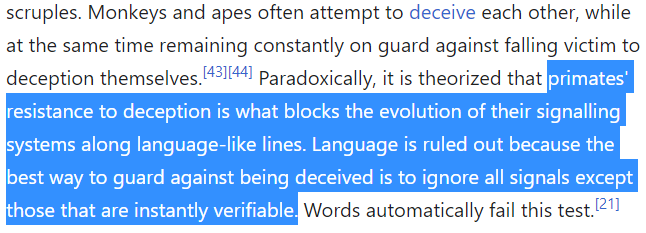
\includegraphics[scale=1.05]{pics/M4/cheaptalkmonke.png}
	\medskip
	
	\url{https://en.wikipedia.org/wiki/Origin_of_language\#Problems_of_reliability_and_deception}
\end{frame}


\begin{frame}{Idea}
	\begin{columns}
		\begin{column}{0.5\textwidth}
			\begin{center}
				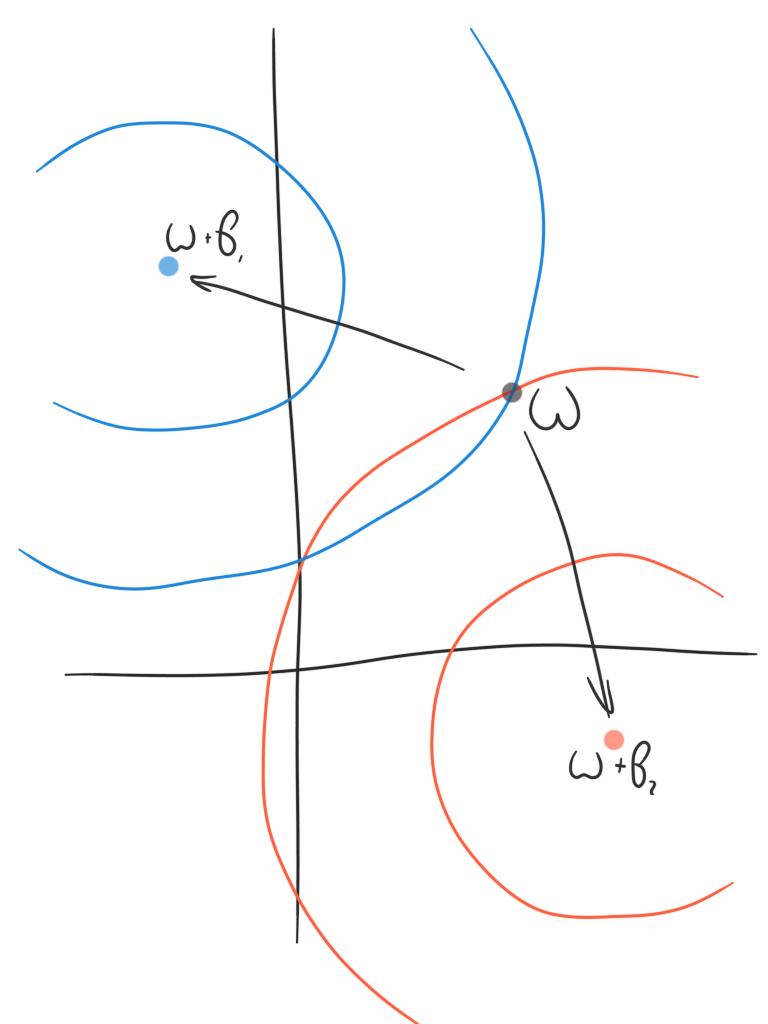
\includegraphics[scale=0.65]{pics/M4/battaglini01.png}
			\end{center}
		\end{column}
		\begin{column}{0.5\textwidth}
			{\small
				\begin{itemize}
					\item Relative positions of bliss points and indifference curves are fixed; just the absolute location unknown.
					\item The circles on the graph represent the indifference curves of the two players.
				\end{itemize}
			}
		\end{column}
	\end{columns}
\end{frame}


\begin{frame}{Idea}
	\begin{columns}
		\begin{column}{0.5\textwidth}
			\begin{center}
				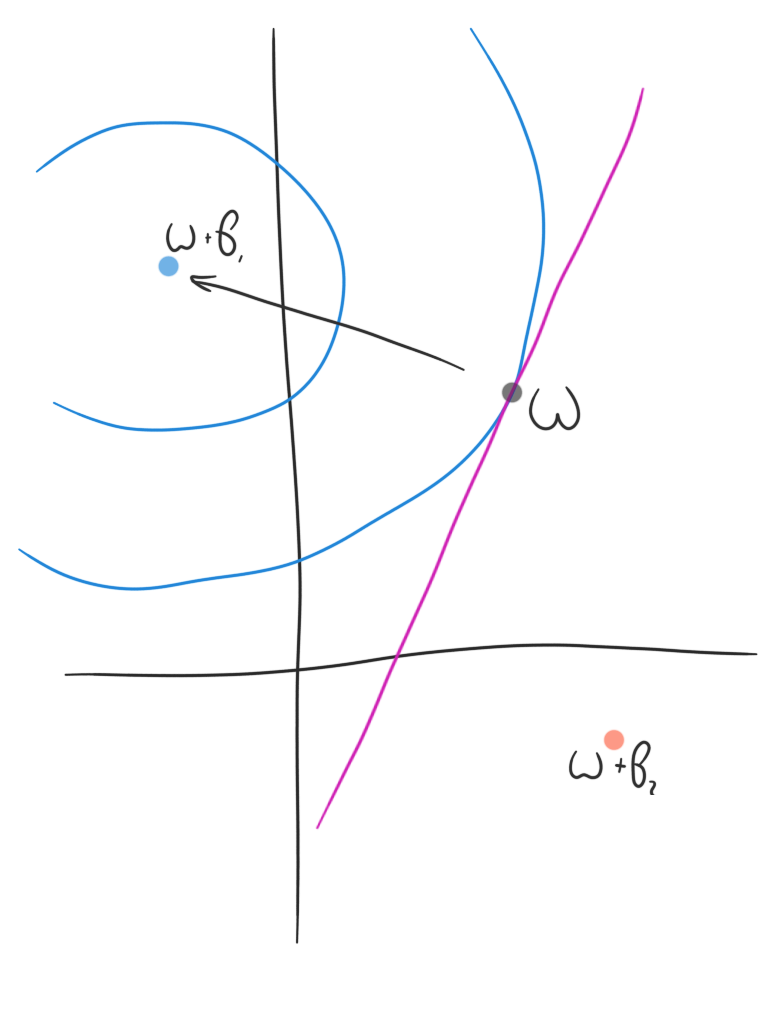
\includegraphics[scale=0.65]{pics/M4/battaglini02.png}
			\end{center}
		\end{column}
		\begin{column}{0.5\textwidth}
			{\small
				\begin{itemize}
					\item Ask player $i$ to project the state on some axis orthogonal to $b_i$ and report the result.
					\item Will report honestly (i.e., report, which is a projection of $\omega +b_1$, coincides with the projection of the actual $\omega$).
					\item So we learn one coordinate of the true state.
				\end{itemize}
			}
		\end{column}
	\end{columns}
\end{frame}


\begin{frame}{Idea}
	\begin{columns}
		\begin{column}{0.5\textwidth}
			\begin{center}
				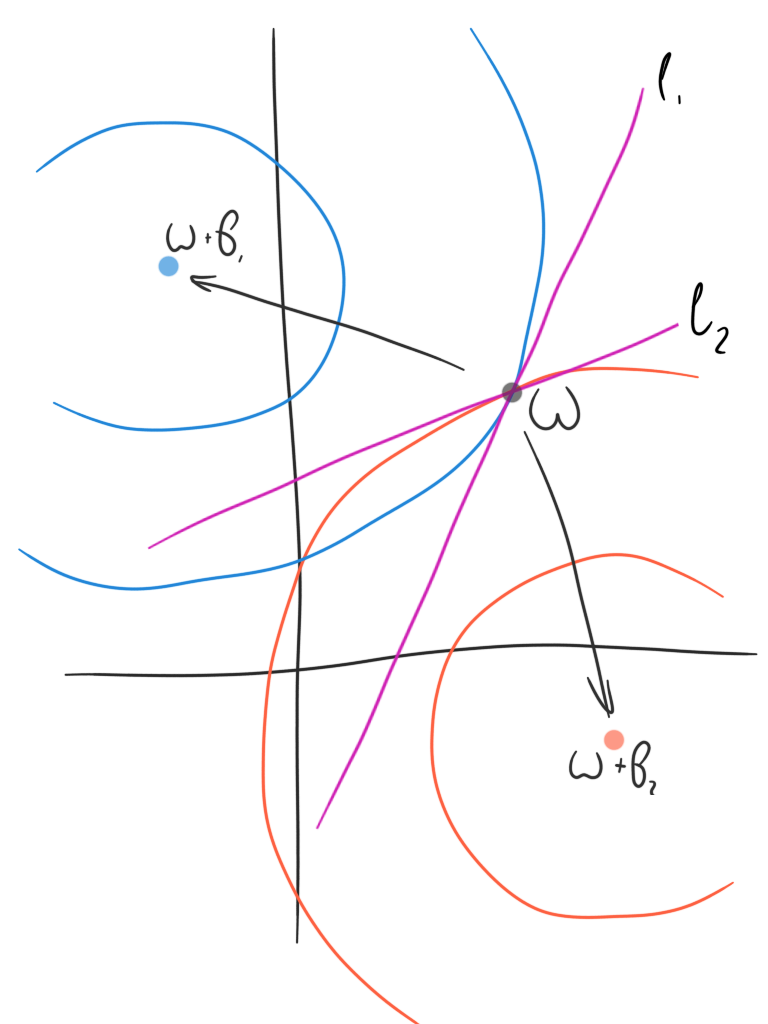
\includegraphics[scale=0.65]{pics/M4/battaglini03.png}
			\end{center}
		\end{column}
		\begin{column}{0.5\textwidth}
			{\small
				\begin{itemize}
					\item Then with two players, we can learn state perfectly this way.
					\item (As long as $b_i$ \structure{linearly independent}.)
					\item More generally, two players are enough to learn the state of any dimensionality $n$, since asking either player allows to learn $n-1$ dimensions of state.
					\item See Battaglini (2002) for $n$ dimensions and more general preferences.
				\end{itemize}
			}
		\end{column}
	\end{columns}
\end{frame}


\begin{frame}{Equilibrium strategies}
	\begin{columns}
		\begin{column}{0.5\textwidth}
			\begin{center}
				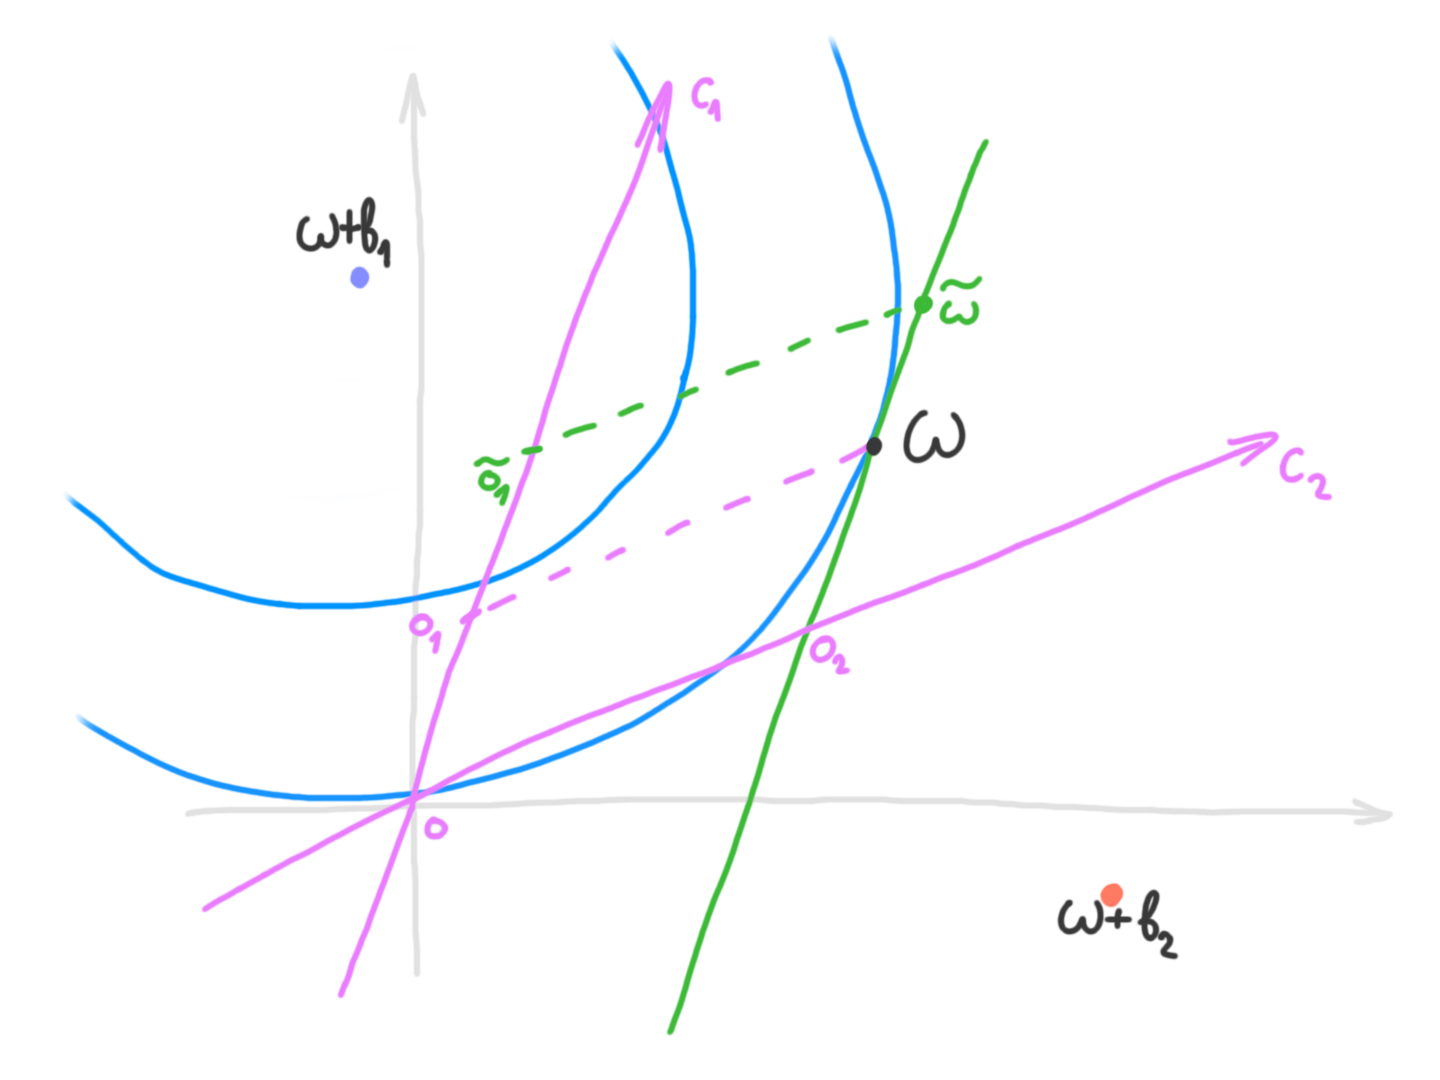
\includegraphics[scale=0.65]{pics/M4/battaglini04.png}
			\end{center}
		\end{column}
		\begin{column}{0.5\textwidth}
			{\small
				\begin{itemize}
					\item Consider basis $(c_1,c_2)$ where $b_i \perp c_i \in \mathbb{R}^2$ -- i.e., $b_i \cdot c_i = 0$ ($\iff b_i^1 c_i^1 + b_i^2 c_i^2 = 0$). 
					\item State $\omega$ has unique coordinates $(o_1,o_2)$ in this basis, i.e. $\omega = o_1 \cdot c_1 + o_2 \cdot c_2$.
					\item Ask A1 to report $o_1$. If A2 reports $o_2$ truthfully, A1 effectively chooses an action on the green line (see graph). 
					\item So truthful reporting is optimal for A1 (green line is orthog to $b_1$ $\Rightarrow$ it is tangent to A1's circular indifference curve at $\omega$ $\Rightarrow$ any lies $\tilde{o}_1$ puts the implemented action $\tilde{\omega}$ on a lower indiff curve).
				\end{itemize}
			}
		\end{column}
	\end{columns}
\end{frame}


\begin{frame}{Clarifications}
	\begin{itemize}
		\item There are many vectors $c_i$ that are orthogonal to a given $b_i$ -- select any.
		\begin{itemize}
			\item E.g., letting $c_i = \frac{1}{\left\| b_i \right\|_2 } \left[ \begin{array}{c c} 0 & 1 \\ -1 & 0 \end{array} \right] \left( \begin{array}{c}
				b_i^1 \\ b_i^2
			\end{array} \right)$ would yield a vector $c_i$ of unit length that is rotated $90\deg$ clockwise w.r.t. $b_i$.
		\end{itemize}
		\item Formally, the problem setup says that messages are two-dimensional: $m_i \in \mathbb{R}^2$. So to be 100\% formal you can say that, e.g., $m_i = (o^i, 0)$, and that the principal ignores the second coordinate of each message.
		\begin{itemize}
			\item Alternatively: agents are expected to report $\omega$, but then the principal calculated respective $o_i$ and decides based on them (even (especially!) if reports do not coincide).
		\end{itemize}
	\end{itemize}
\end{frame}



\section{Example 5: Dynamic }

\begin{frame}{title}
content...
\end{frame}


\appendix
\begin{frame}[allowframebreaks]{References}
\bibliography{teaching}
\bibliographystyle{abbrvnat}
\end{frame}


\end{document}